\section{Moltres Spalart-Allmaras Turbulence Model Verification} \label{sec:turbulence}

As detailed in Section \ref{sec:th}, Moltres compiles with the MOOSE Navier-Stokes
\cite{peterson_overview_2018} and Heat Transfer modules for incompressible flow
modeling capabilities by default. Moltres couples with these modules natively because they are all
built on the MOOSE framework.

To address the lack of turbulence modeling in Moltres, I implemented a \gls{SA} turbulence model
\cite{spalart_one-equation_1994}, described in Section \ref{sec:lit-turb}, with \gls{SUPG}
stabilization on Moltres. The \gls{SA} model estimates the turbulent eddy viscosity defined by the
eddy viscosity hypothesis applied to the \gls{RANS} equations \cite{rodi_turbulence_2017}.
On balance the \gls{SA} model is a complete (does not require prior
knowledge of the actual turbulence behavior) and computationally efficient one-equation turbulence
model for approximating wall-bounded turbulent flows. The \gls{SA} model implementation in Moltres
couples seamlessly with the continuous \gls{FEM} \gls{INSAD}
\cite{peterson_overview_2018, lindsay_automatic_2021} model
from the Navier-Stokes module. Alongside the \gls{SA} model, Moltres also now has turbulent
diffusion physics kernels for temperature and the delayed neutron precursors.

The SA model in Moltres follows the \gls{SA} model with a rotation correction scheme
\cite{aupoix_extensions_2003, dacles-mariani_numericalexperimental_1995} as described on the
\gls{NASA} Turbulence Modeling Resource website \cite{rumsey_turbulence_nodate}. The rotation
correction reduces eddy viscosity in regions of rotational but non-turbulent flow where the
original \gls{SA} model overestimates eddy viscosity. The \gls{SA} model implementation in Moltres
solves for the modified dynamic viscosity $\tilde{\mu}$ (as opposed to $\tilde{\nu}$) as follows:

\begin{gather}
  \rho \frac{\partial\tilde{\mu}}{\partial t} + \rho \mathbf{u}\cdot\nabla\tilde{\mu} = \rho c_{b1}
  \left(1-f_{t2}\right)\tilde{S}\tilde{\mu} + \frac{1}{\sigma}\{\nabla\cdot\left[\left(\mu+
  \tilde{\mu}\right)\nabla\tilde{\mu}\right] + c_{b2}|\nabla\tilde{\mu}|^2\} - \left(c_{w1}f_w -
  \frac{c_{b1}}{\kappa^2}f_{t2}\right)\left(
  \frac{\tilde{\mu}}{d}\right)^2
  \shortintertext{where}
  \begin{align*}
    \mu_t &= \tilde{\mu}f_{v1} = \text{turbulent eddy viscosity}, &
    f_{v1} &= \frac{\chi^3}{\chi^3 + c_{v1}^3}, \\
    \chi &= \frac{\tilde{\mu}}{\mu}, &
    \tilde{S} &= \Omega + \frac{\tilde{\nu}}{\kappa^2 d^2} f_{v2}, \\
    f_{v2} &= 1 - \frac{\chi}{1+\chi f_{v1}}, &
    \Omega &= \sqrt{2W_{ij}W_{ij}} = \text{vorticity magnitude}, \\
    W_{ij} &= \frac{1}{2}\left(\frac{\partial u_i}{\partial x_j} - \frac{\partial u_j}{\partial x_i}
    \right), &
      f_w &= g\left(\frac{1 + c_{w3}^6}{g^6 + c_{w3}^6}\right)^{1/6}, \\
      g &= r + c_{w2}\left(r^6 - r\right), &
      r &= \text{min}\left(\frac{\tilde{\nu}}{\tilde{S}\kappa^2d^2}, 10\right), \\
      f_{t2} &= c_{t3} \exp{\left(-c_{t4}\chi^2\right)},
  \end{align*}
\shortintertext{and the constants are}
  \sigma = \frac{2}{3}, \ c_{b1} = 0.1355, \ c_{b2} = 0.622, \ \kappa = 0.41, \
  c_{w1} = \frac{c_{b1}}{\kappa^2} + \frac{1+c_{b2}}{\sigma}, \nonumber \\
  c_{w2} = 0.3, \ c_{w3} = 2, \
  c_{v1} = 7.1, \ c_{t3} = 1.2, \ c_{t4} = 0.5 \ \text{.} \nonumber
\end{gather}

The $f_{t2}$ turbulence trip term is togglable using the \texttt{use\_ft2\_term} input parameter
(false by default) if turbulence trip (initiation) is not necessary
\cite{rumsey_turbulence_nodate}. The following subsections cover verification and validation tests
of the \gls{SA} model in Moltres using reference problems for turbulent channel, pipe, and
\gls{BFS} flow. Moltres input files
for all three reference problems are available at
\url{https://github.com/arfc/moltres/tree/devel/problems/2023-basic-turbulence-cases}.
The Moltres test dataset is available on Zenodo at this reference listing \cite{park_dataset_2023}.

\subsection{Turbulent Channel Flow Verification Test}

Moser et al.\ \cite{moser_direct_1999} performed \gls{DNS} simulations of turbulent channel flow
for friction Reynolds number, Re$_\tau\approx395$ (corresponds to Reynolds number, Re
$\approx 13750$). Their results serve as the reference solution for this turbulent channel flow
test.

The Moltres model for this test is a 2-D 140 m$\times$0.5 m half-channel. The main flow direction
is in the positive $x$ direction with the inlet and outlet on the left and right ends,
respectively. The channel wall lies along the top boundary ($y=0.5$ m) while the bottom boundary
($y=0$ m) serves as a symmetry axis for the half-channel geometry. Figure \ref{fig:channel-mesh}
shows a close-up view of the refined mesh near the inlet and along the top wall boundary. The mesh
for the rest of the channel geometry follows the same mesh resolution as the rightmost column of
elements shown on the right side of Figure \ref{fig:channel-mesh}. The dimensionless wall distance
parameter $y^+$ of the first mesh element along wall boundary for fully developed flow at the end
of the channel is 0.974, meeting the
$y^+ \lesssim 1$ requirement for properly wall-resolved flow. Table \ref{table:channel} lists
relevant flow parameters for the turbulent channel flow test. The Moltres channel flow model
ran as a time-dependent simulation with adaptive time-stepping starting from a timestep size of 0.1
s up to a maximum timestep size of 10 s with a timestep size growth factor of 1.1. The simulation
automatically terminated at $t=186$ s when Moltres detected that the flow profile reached
steady-state, i.e., the flow and turbulent viscosity distributions remained unchanged between
successive timesteps.

\begin{figure}[htb!]
  \centering
  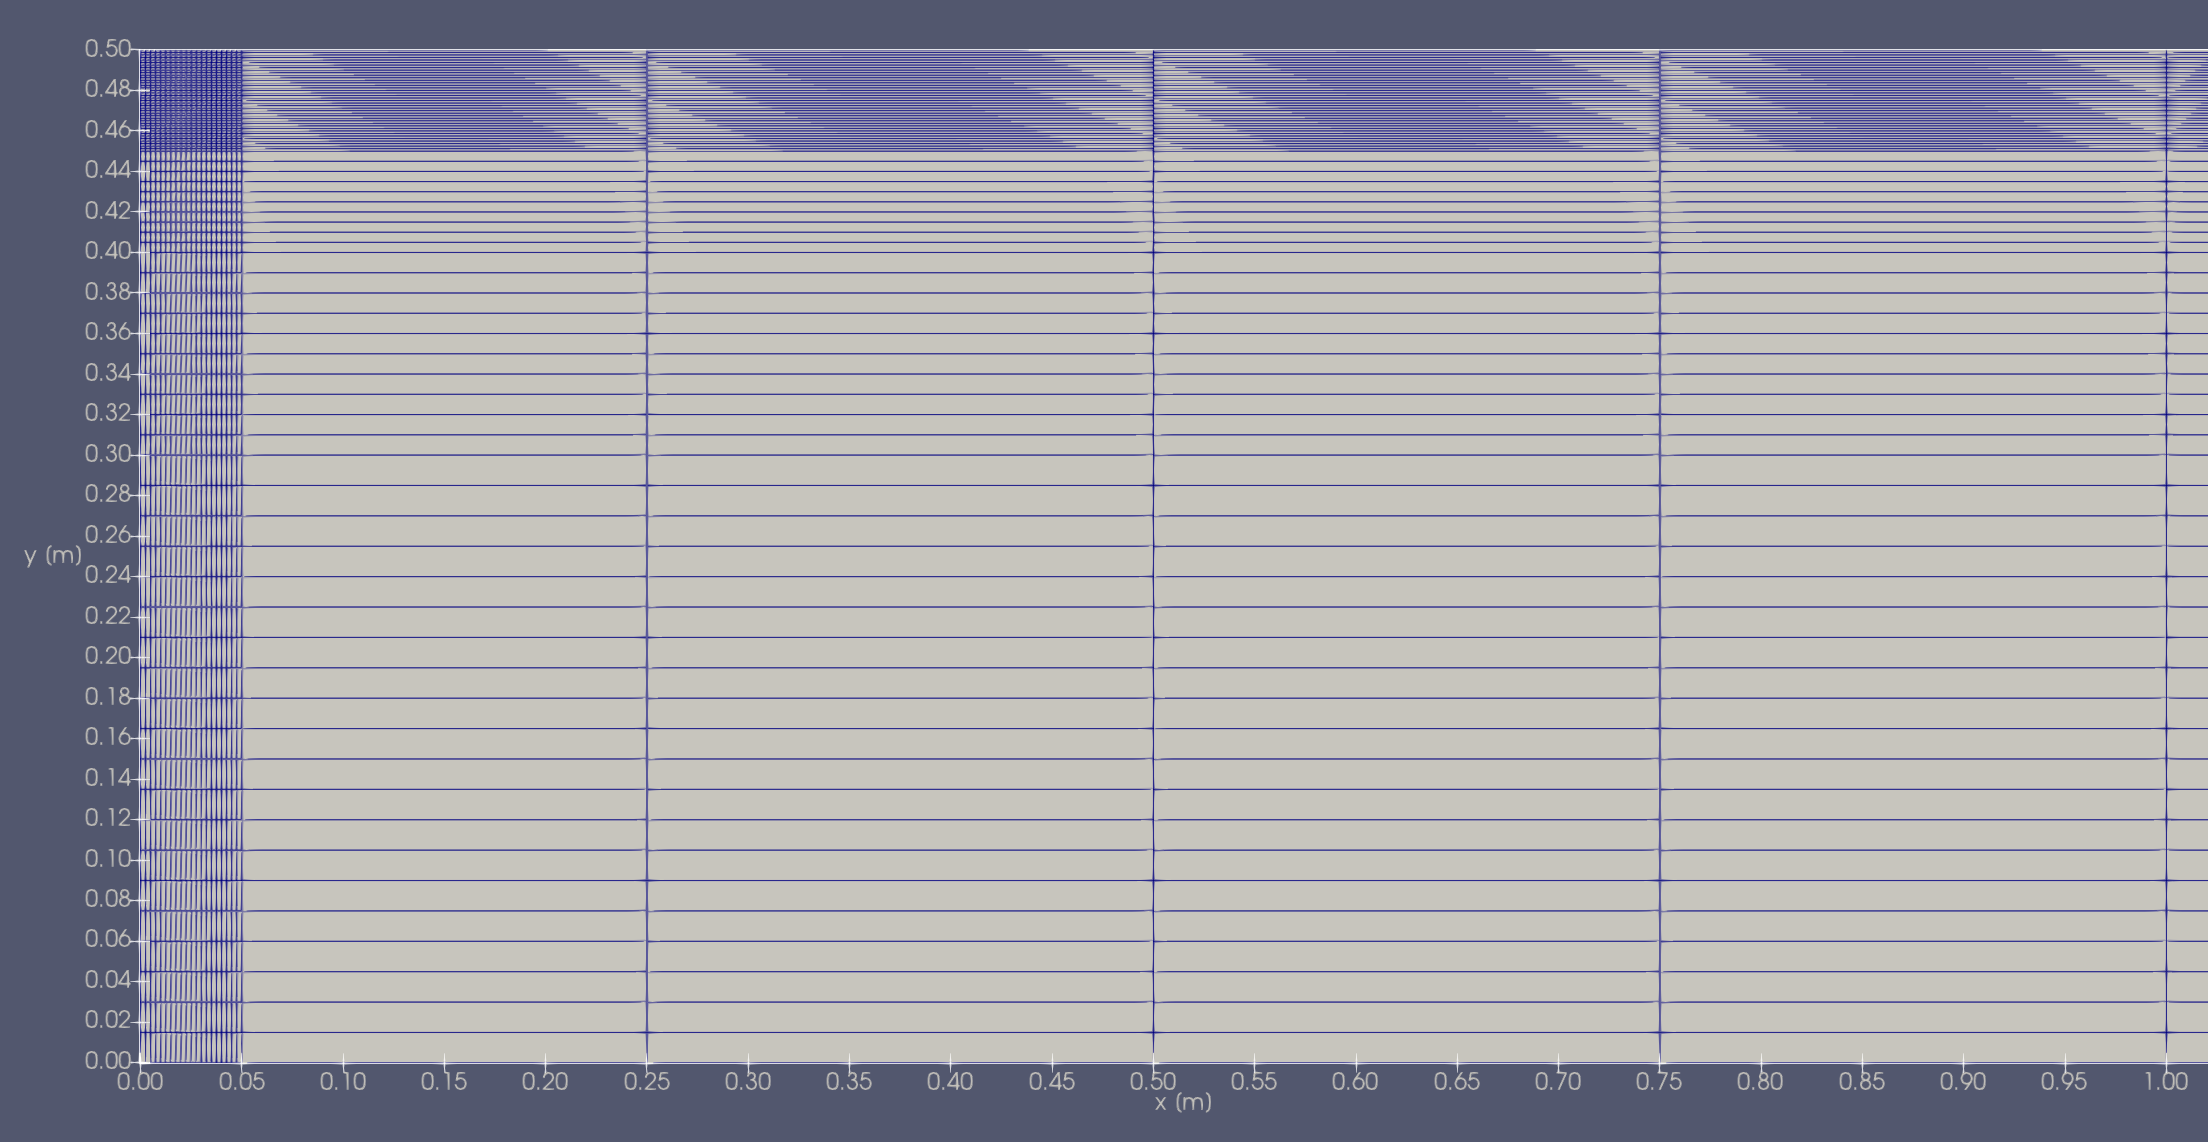
\includegraphics[width=\columnwidth]{channel_mesh}
  \caption{Close-up view of the refined mesh near the inlet (left boundary) for the channel flow
    test. The mesh for the rest of the channel follows the mesh resolution of the rightmost column
  of elements.}
  \label{fig:channel-mesh}
\end{figure}

\begin{table}[htb]
  \centering
  \small
  \caption{Relevant turbulent channel flow problem parameters. The $\tilde{\mu}_\text{inlet}$ value
  at the inlet is set to fives times the $\mu$ value as recommended for the \gls{SA} model
  \cite{spalart_one-equation_1994}.}
  \begin{tabular}{l S}
    \toprule
    Property & {Value} \\
    \midrule
    Density, $\rho$ [kg m$^{-3}$] & 1.0 \\
    Inlet velocity, $v_x$ [m s$^{-1}$] & 1.0 \\
    Dynamic viscosity, $\mu$ [kg m$^{-1}$ s$^{-1}$] & 7.272e-5 \\
    Reynolds number, Re [-] & 1.375e4 \\
    Modified viscosity along inlet, $\tilde{\mu}_\text{inlet}$ [kg m$^{-1}$ s$^{-1}$] & 3.636e-4 \\
    Modified viscosity along wall, $\tilde{\mu}_\text{wall}$ [kg m$^{-1}$ s$^{-1}$] & 0.0 \\
    \bottomrule
  \end{tabular}
  \label{table:channel}
\end{table}

Figure \ref{fig:channel-verification} shows plots of normalized and nondimensionalized velocities,
wall distances, and stresses from the \gls{DNS} data \cite{moser_direct_1999}
and the Moltres \gls{SA} model. The Moltres \gls{SA} model is largely consistent with the reference
\gls{DNS} flow data and reproduces the expected trends in the velocity and stress distributions
across the channel and as a function of the wall distance.

\begin{figure}[htb!]
  \centering
  \begin{subfigure}[b]{0.48\columnwidth}
    \centering
    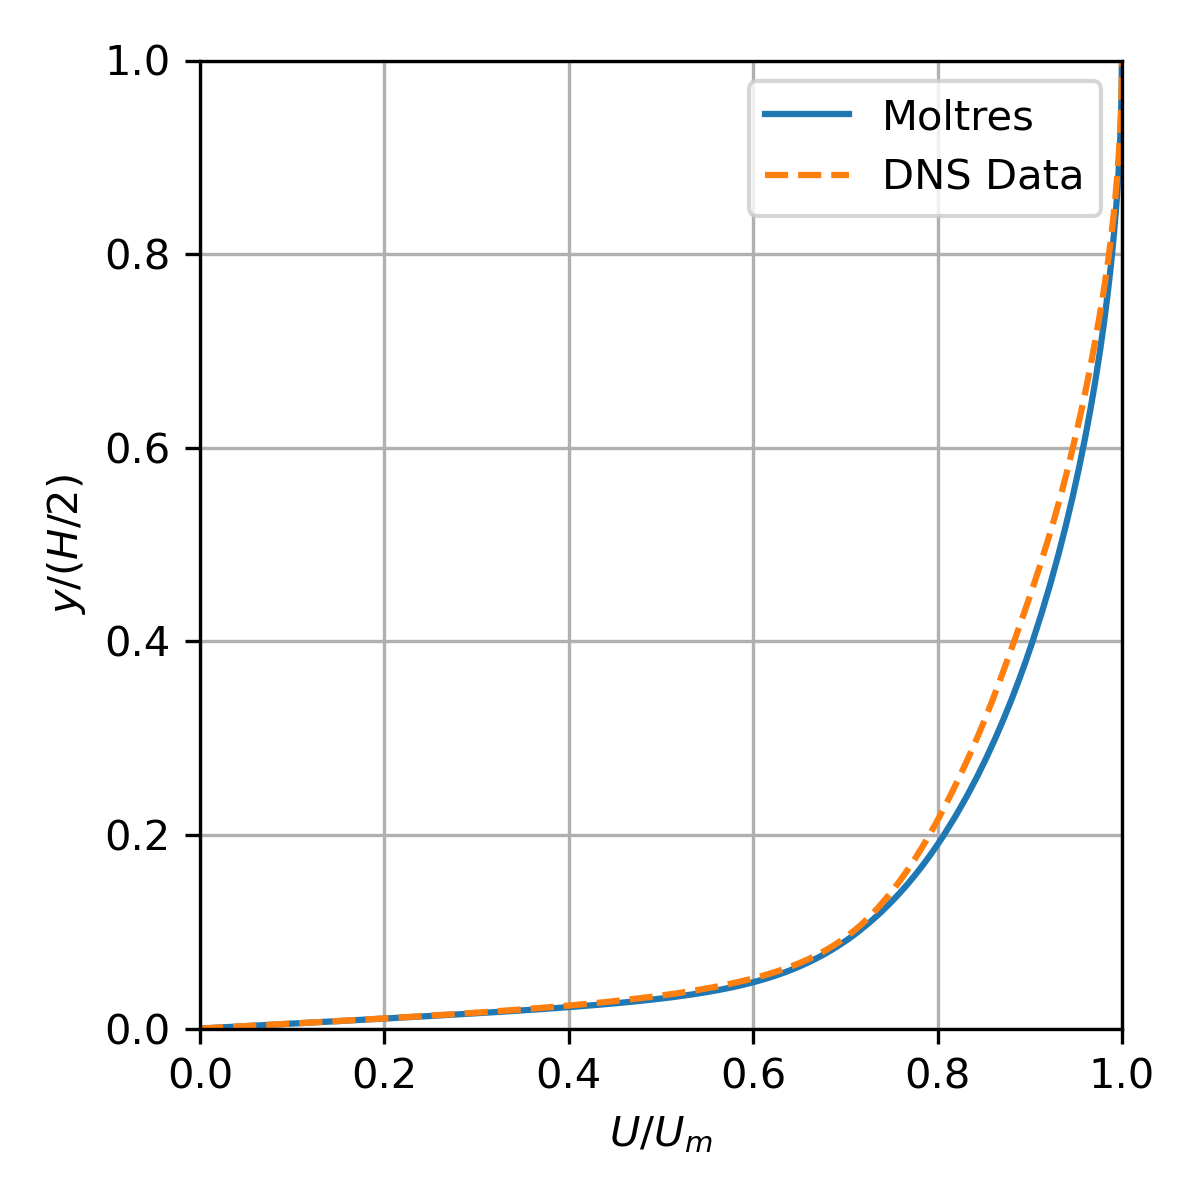
\includegraphics[width=\columnwidth]{channel_vel}
    \caption{Normalized velocity distribution across the channel.}
    \label{fig:channel-vel}
  \end{subfigure}
  \hfill
  \begin{subfigure}[b]{0.48\columnwidth}
    \centering
    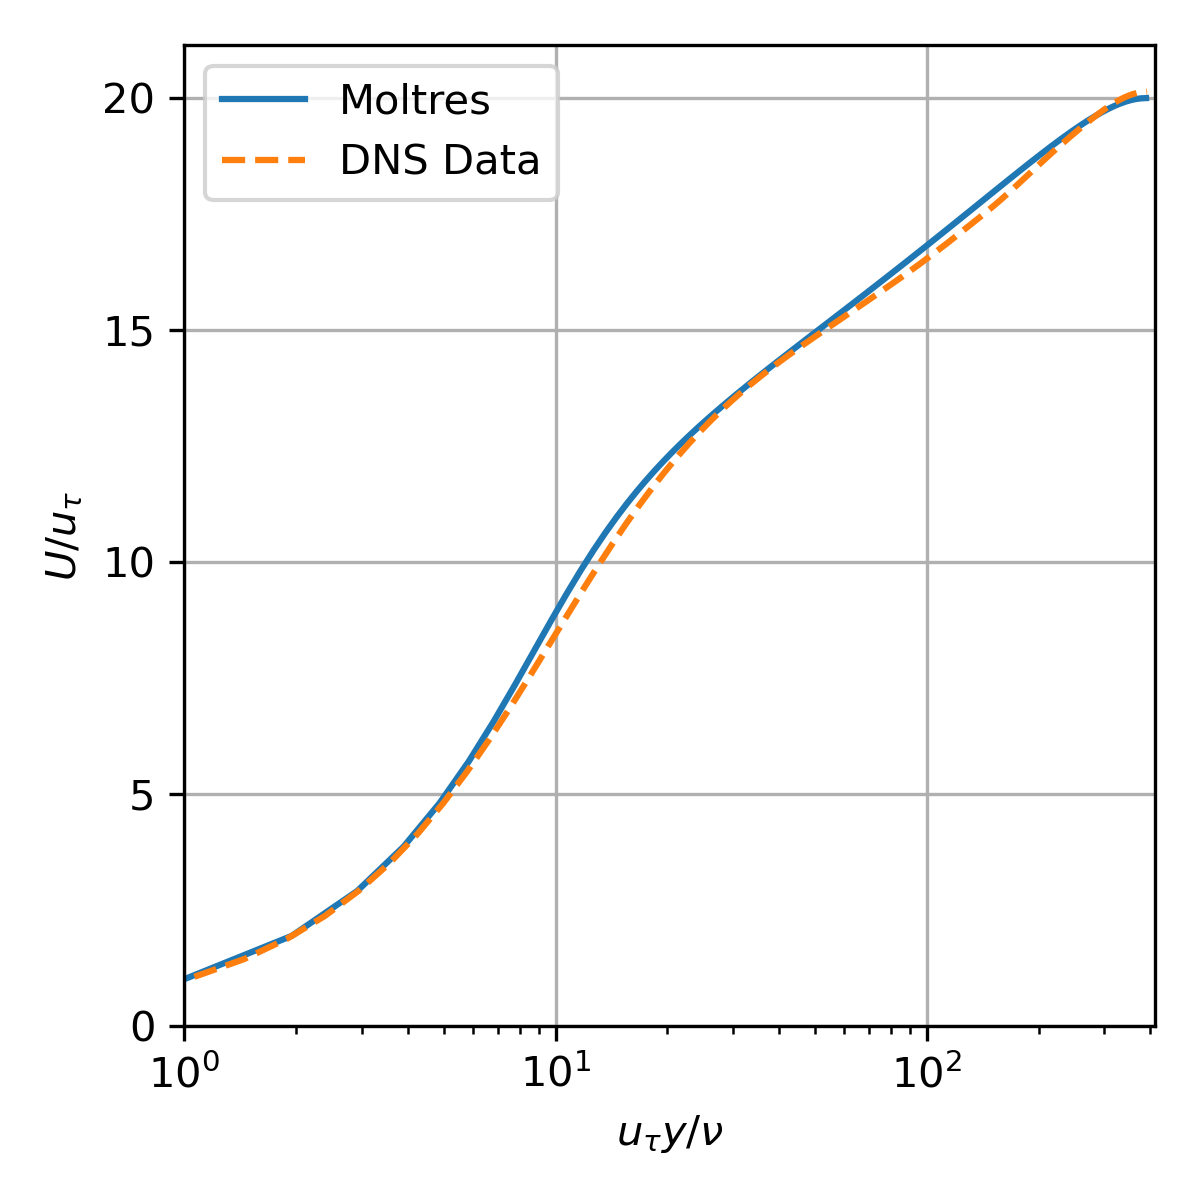
\includegraphics[width=\columnwidth]{channel_nondim}
    \caption{Dimensionless velocity vs.\ dimensionless wall distance.}
    \label{fig:channel-nondim}
  \end{subfigure}
  \begin{subfigure}[b]{0.48\columnwidth}
    \centering
    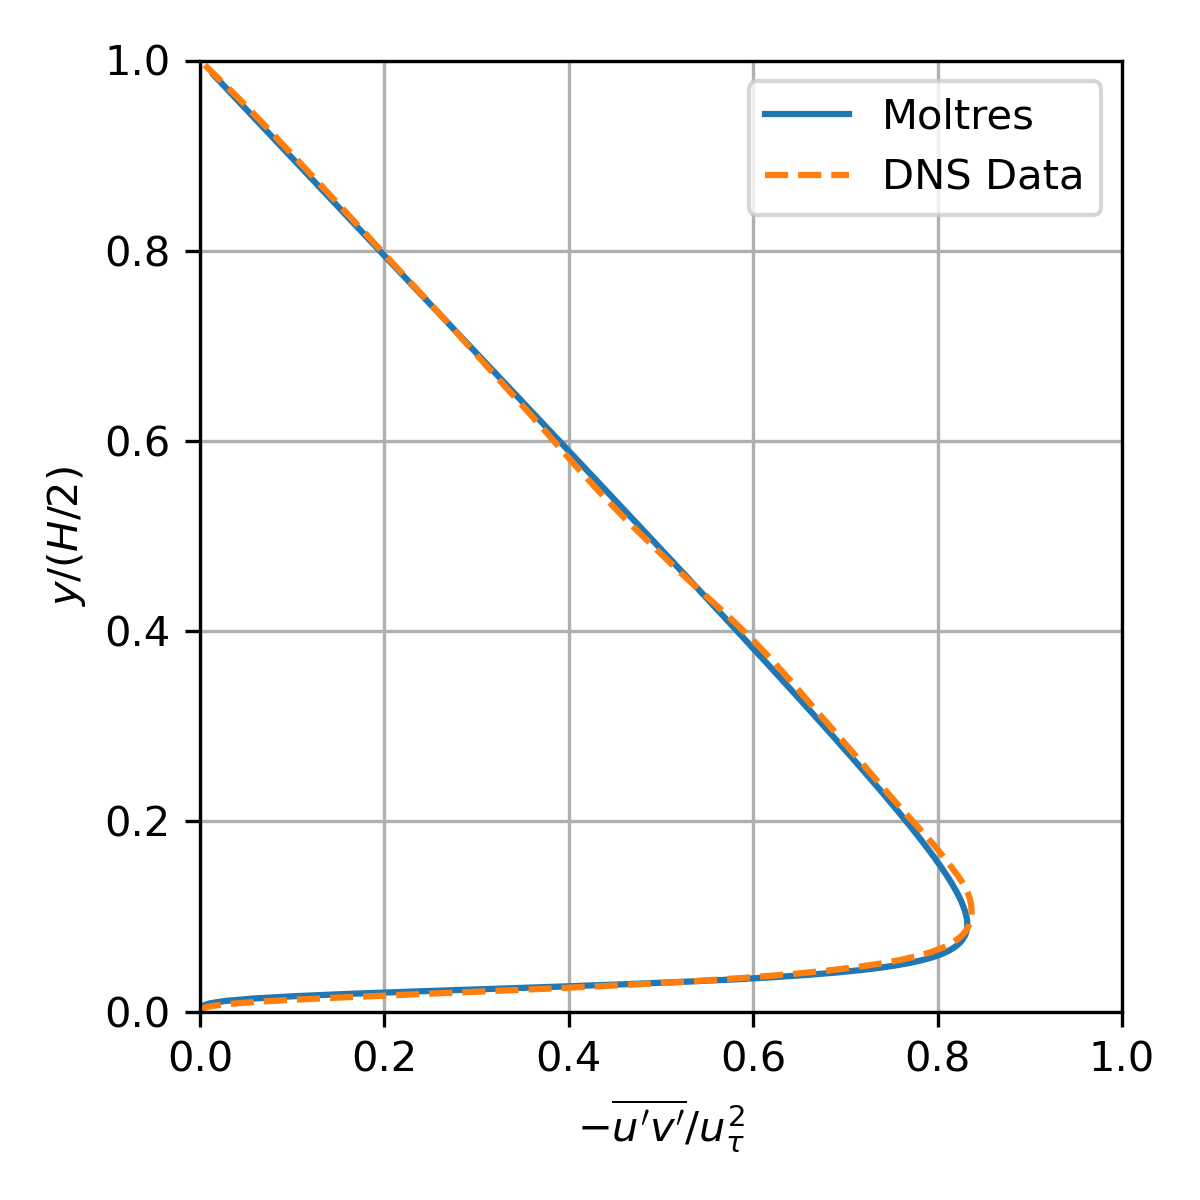
\includegraphics[width=\columnwidth]{channel_stress}
    \caption{Normalized stress distribution across the channel.}
    \label{fig:channel-stress}
  \end{subfigure}
  \caption{Comparison of turbulent channel flow results at Re$_\tau\approx395$ against reference
  \gls{DNS} results \cite{moser_direct_1999}. The Moltres \gls{SA} model agrees consistently with
  the reference data.}
  \label{fig:channel-verification}
\end{figure}

\subsection{Turbulent Pipe Flow Validation Test}

In 1954, Laufer performed turbulent pipe flow experiments for Re $\approx 40000$
\cite{laufer_structure_1954}. Their results serve as the reference solution for this turbulent pipe
flow test.

\begin{figure}[htb!]
  \centering
  \begin{subfigure}[b]{0.42\columnwidth}
    \centering
    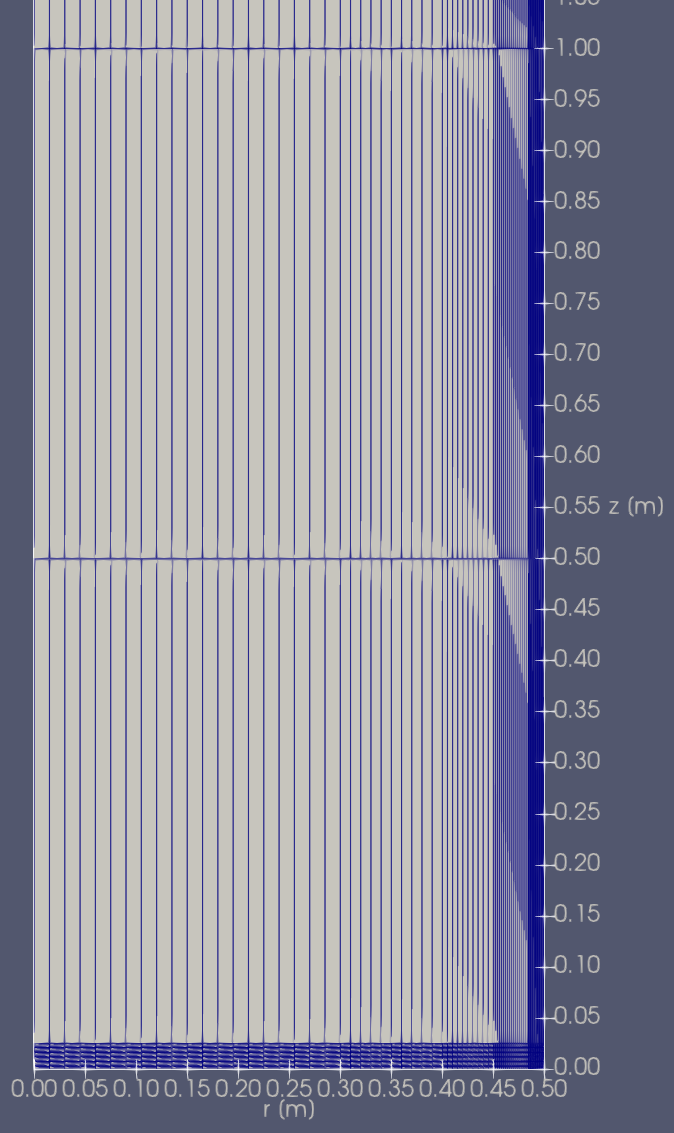
\includegraphics[width=\columnwidth]{pipe_mesh}
    \caption{Close-up view of the refined mesh near the inlet for the pipe flow test.}
    \label{fig:pipe-mesh-1}
  \end{subfigure}
  \hfill
  \begin{subfigure}[b]{0.56\columnwidth}
    \centering
    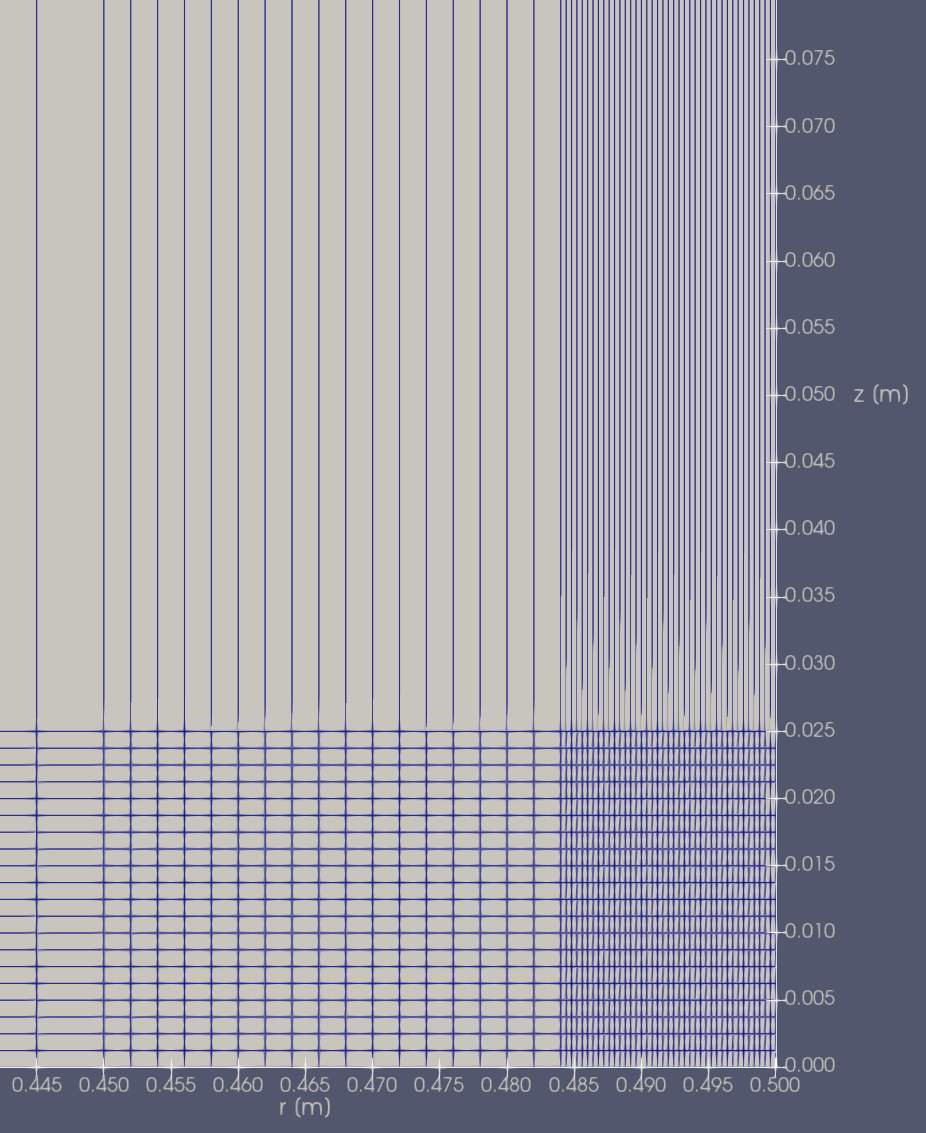
\includegraphics[width=\columnwidth]{pipe_mesh_zoom}
    \caption{Close-up view of the refined mesh near the inlet and wall boundary interface.}
    \label{fig:pipe-mesh-2}
  \end{subfigure}
  \caption{Close-up views of the refined mesh near the inlet (bottom boundary) and wall (right
  boundary). The mesh for the rest of the channel follows the mesh resolution of the topmost row of
  elements in the left subfigure.}
  \label{fig:pipe-mesh}
\end{figure}

The Moltres model for this test is a 2-D axisymmetric (R-Z coordinates) half-pipe with a radius of
0.5 m and a length of 150 m. The main flow direction
is in the positive $z$ direction with the inlet and outlet on the bottom and top ends,
respectively. The channel wall lies along the right boundary ($r=0.5$ m) while the left boundary
($r=0$ m) serves as a symmetry axis for the half-pipe geometry. Figure \ref{fig:pipe-mesh} shows
two close-up views of the refined mesh near the inlet and along the right wall boundary. The mesh
for the rest of the pipe geometry follows the same mesh resolution as the topmost row of
elements shown on the near the top of Figure \ref{fig:pipe-mesh-1}. The dimensionless wall distance
parameter $y^+$ of the first mesh element along wall boundary for fully developed flow at the end
of the pipe is 0.847, meeting the
$y^+ \lesssim 1$ requirement for properly wall-resolved flow. Table \ref{table:channel} lists
relevant flow parameters for the turbulent pipe flow test. The Moltres channel flow model ran as a
time-dependent simulation with adaptive time-stepping starting from a timestep size of 0.01
s up to a maximum timestep size of 10 s with a timestep size growth factor of 1.1. The simulation
automatically terminated at $t=165$ s when Moltres detected that the flow profile reached
steady-state, i.e., the flow and turbulent viscosity distributions remained unchanged between
successive timesteps.

\begin{table}[htb]
  \centering
  \small
  \caption{Relevant turbulent pipe flow problem parameters. The $\tilde{\mu}_\text{inlet}$ value
  at the inlet is set to fives times the $\mu$ value as recommended for the \gls{SA} model
  \cite{spalart_one-equation_1994}.}
  \begin{tabular}{l S}
    \toprule
    Property & {Value} \\
    \midrule
    Density, $\rho$ [kg m$^{-3}$] & 1.0 \\
    Inlet velocity, $v_z$ [m s$^{-1}$] & 1.0 \\
    Dynamic viscosity, $\mu$ [kg m$^{-1}$ s$^{-1}$] & 2.5e-5 \\
    Reynolds number, Re [-] & 4.0e4 \\
    Modified viscosity along inlet, $\tilde{\mu}_\text{inlet}$ [kg m$^{-1}$ s$^{-1}$] & 1.25e-4 \\
    Modified viscosity along wall, $\tilde{\mu}_\text{wall}$ [kg m$^{-1}$ s$^{-1}$] & 0.0 \\
    \bottomrule
  \end{tabular}
  \label{table:pipe}
\end{table}

Figure \ref{fig:pipe-verification} shows plots of normalized and nondimensionalized velocities,
wall distances, and stresses from the experimental data \cite{laufer_structure_1954}
and the Moltres \gls{SA} model. The Moltres \gls{SA} model is largely consistent with the reference
experimental flow data and reproduces the expected trends in the velocity and stress distributions
across the channel and as a function of the wall distance.

\begin{figure}[htb]
  \centering
  \begin{subfigure}[b]{0.48\columnwidth}
    \centering
    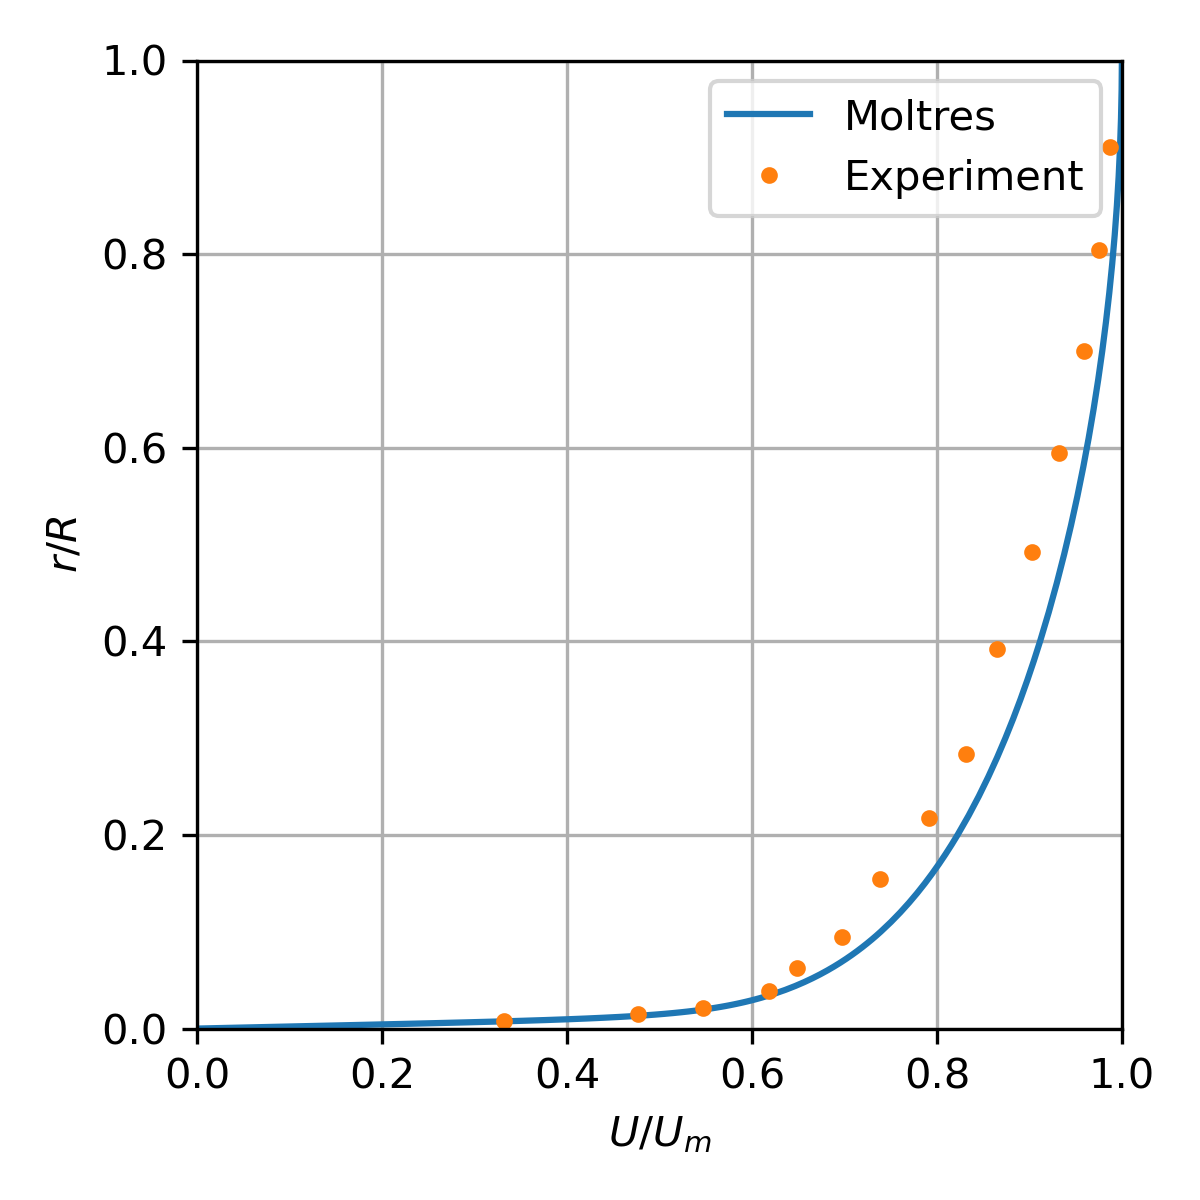
\includegraphics[width=\columnwidth]{pipe_vel}
    \caption{Normalized velocity distribution across the pipe.}
    \label{fig:pipe-vel}
  \end{subfigure}
  \hfill
  \begin{subfigure}[b]{0.48\columnwidth}
    \centering
    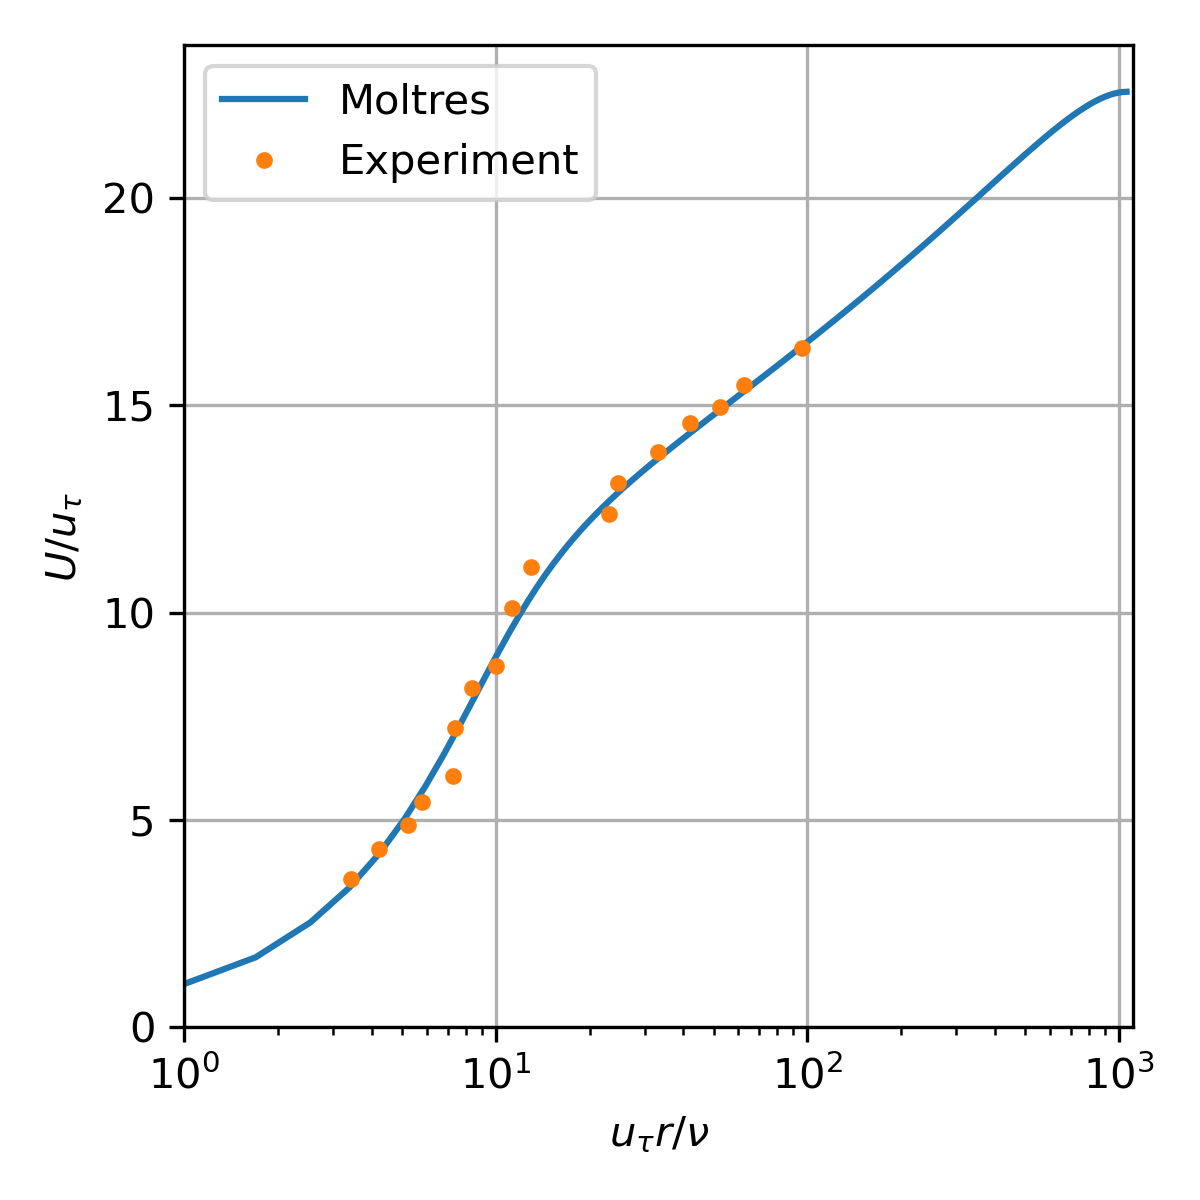
\includegraphics[width=\columnwidth]{pipe_nondim}
    \caption{Dimensionless velocity vs.\ dimensionless wall distance}
    \label{fig:pipe-nondim}
  \end{subfigure}
  \begin{subfigure}[b]{0.48\columnwidth}
    \centering
    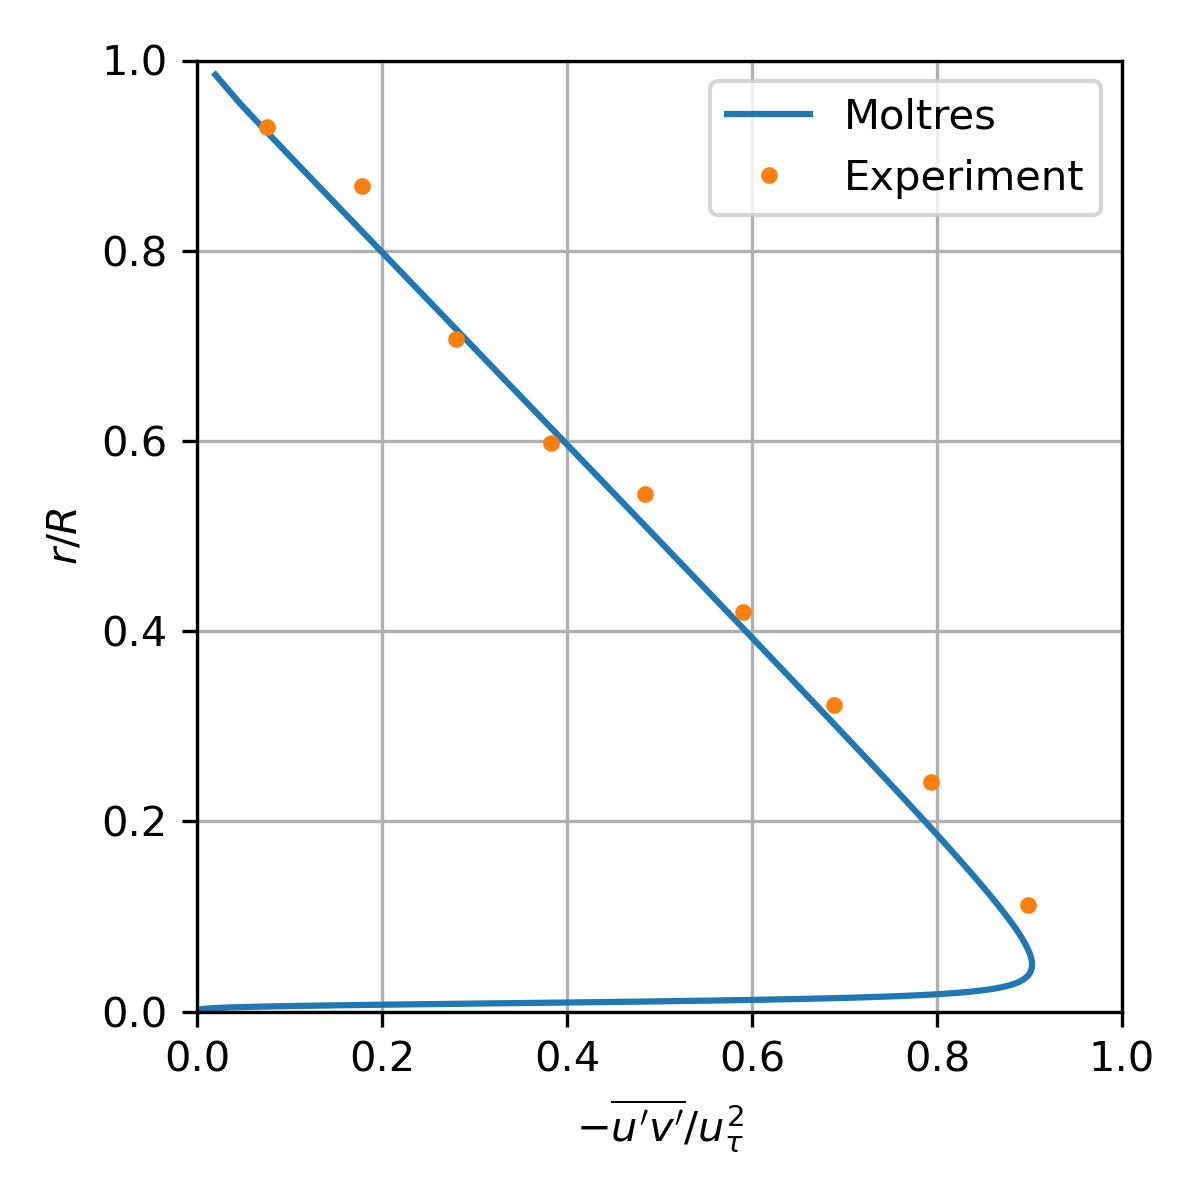
\includegraphics[width=\columnwidth]{pipe_stress}
    \caption{Normalized turbulent shear stress distribution across the pipe.}
    \label{fig:pipe-stress}
  \end{subfigure}
  \caption{Comparison of turbulent pipe flow results at Re $\approx 40000$ against reference
  experimental data \cite{laufer_structure_1954}.}
  \label{fig:pipe-verification}
\end{figure}

\FloatBarrier

\subsection{Backward-Facing Step Flow Validation Test}

Driver \& Seegmiller performed the \gls{BFS} flow experiment for Re $\approx36000$ (based on the
step height)
\cite{driver_features_1985}. Their results serve as the reference solution for this \gls{BFS} test.
Additionally, the \gls{NASA} Turbulence Modeling Resource website \cite{rumsey_turbulence_nodate}
provides \gls{BFS} simulation results generated from the regular \gls{SA} model in the CFL3D
Navier-Stokes CFD code developed at \gls{NASA} \cite{krist_cfl3d_1998}. The CFL3D \gls{SA} model
does not contain the rotation correction scheme
\cite{aupoix_extensions_2003, dacles-mariani_numericalexperimental_1995} present in the Moltres
\gls{SA} model.

\begin{figure}[htb!]
  \centering
  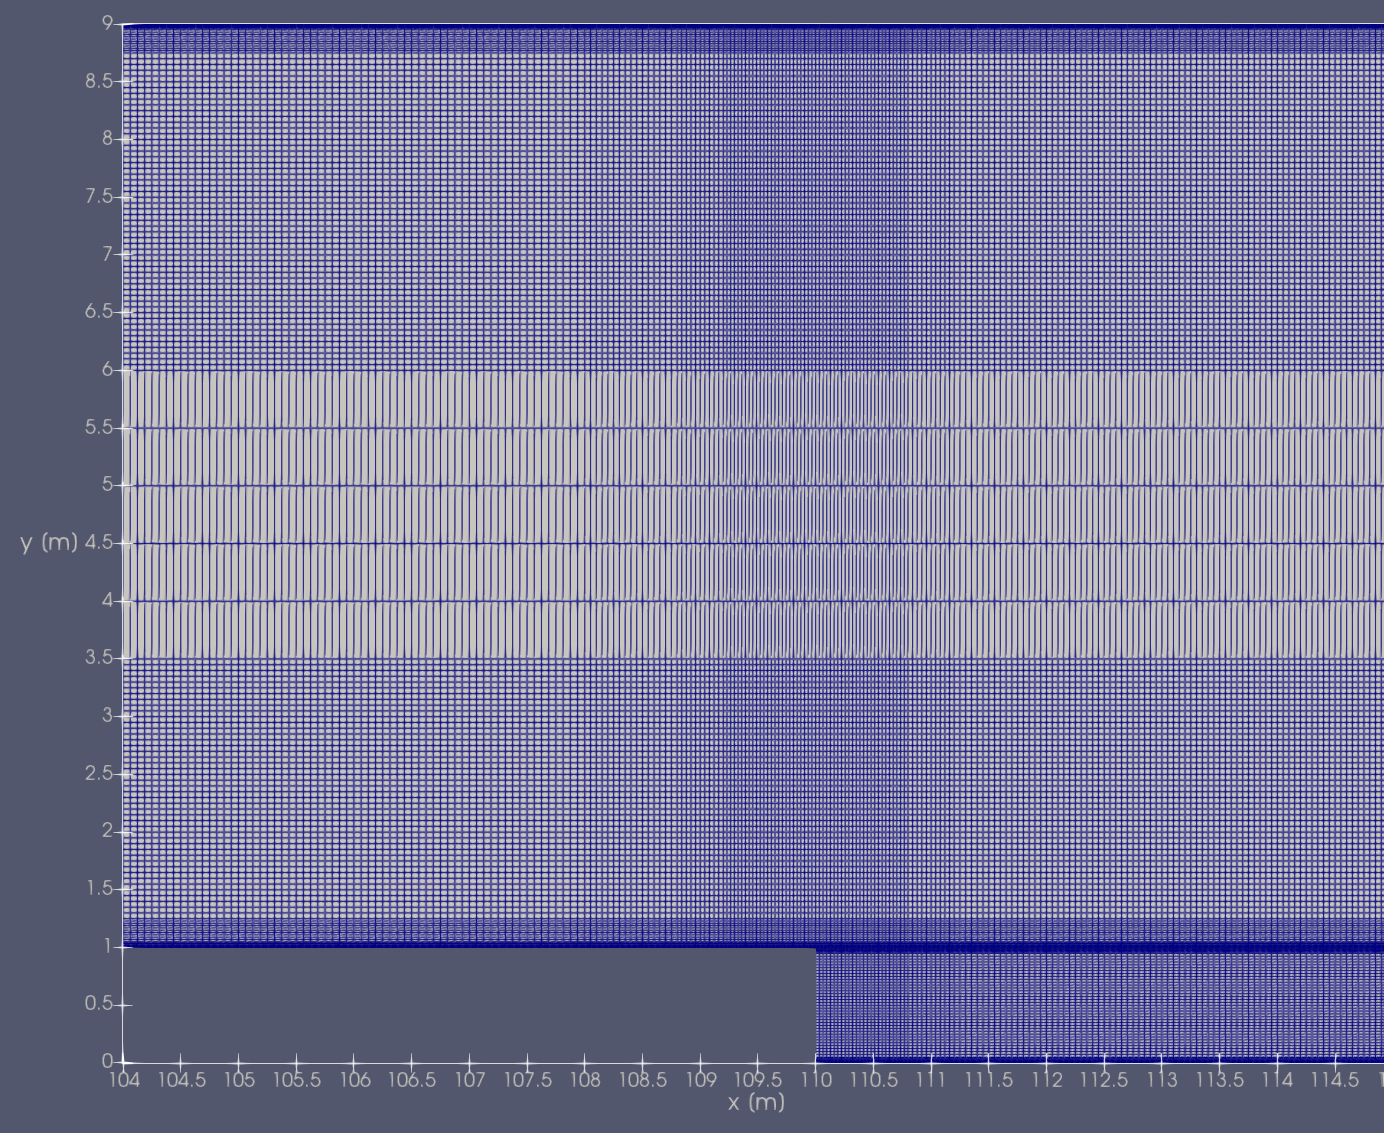
\includegraphics[width=0.9\columnwidth]{bfs_mesh}
  \caption{Close-up view of the mesh for the \gls{BFS} flow test. The step is situated at $x=110$ m
  with a height of $H=1$ m.}
  \label{fig:bfs-mesh}
\end{figure}

The Moltres model for this test is a 2-D 160 m-long channel. The main flow direction is in the
positive $x$ direction with the inlet and outlet on the left and right ends, respectively. The
channel is 8 m tall before the 1 m-tall step at $x=110$ m. Figure \ref{fig:bfs-mesh} shows a
close-up view of the mesh around the step. The dimensionless wall distance parameter $y^+$ of the
first mesh elements along wall boundaries just prior to the step and at the end of the channel are
0.735 and 0.555, respectively, meeting the $y^+ \lesssim 1$ requirement for properly wall-resolved
flow. Table \ref{table:bfs} lists relevant flow parameters for the turbulent \gls{BFS} flow test.
The Moltres \gls{BFS} flow model ran as two separate simulations for the upstream turbulent flow
profile to fully develop from $x=0$ m to $x=104$ m and the \gls{BFS} flow profile from $x=104$ m to
$x=160$ m. The fully-developed flow profile at $x=104$ m from the first simulation served as the
inlet flow profile for the second simulation. Both simulations ran with adaptive time-stepping
starting from a timestep size of 0.1 s up to a maximum timestep size of 10 s with a timestep size
growth factor of 1.1. The upstream and \gls{BFS} simulations automatically terminated at $t=212$ s
and $t=223$ s when Moltres detected that the flow profiles reached steady-state.

\begin{table}[htb]
  \centering
  \small
  \caption{Relevant turbulent \gls{BFS} flow problem parameters. The $\tilde{\mu}_\text{inlet}$ value
  at the inlet is set to fives times the $\mu$ value as recommended for the \gls{SA} model
  \cite{spalart_one-equation_1994}.}
  \begin{tabular}{l S}
    \toprule
    Property & {Value} \\
    \midrule
    Density, $\rho$ [kg m$^{-3}$] & 1.0 \\
    Inlet velocity, $v_z$ [m s$^{-1}$] & 1.0 \\
    Dynamic viscosity, $\mu$ [kg m$^{-1}$ s$^{-1}$] & 2.778e-5 \\
    Reynolds number based on step height $H=1$ m, Re$_H$ [-] & 3.6e4 \\
    Modified viscosity along inlet, $\tilde{\mu}_\text{inlet}$ [kg m$^{-1}$ s$^{-1}$] & 1.389e-4 \\
    Modified viscosity along wall, $\tilde{\mu}_\text{wall}$ [kg m$^{-1}$ s$^{-1}$] & 0.0 \\
    \bottomrule
  \end{tabular}
  \label{table:bfs}
\end{table}

Figure \ref{fig:bfs} shows the velocity magnitude and streamlines around the step at $x=110$ m. The
streamlines illustrate the recirculation zones created by flow separation past the step.
Figure \ref{fig:bfs-plots} shows the normalized velocity distributions at various distances from
step, the skin friction and skin pressure coefficients along the bottom wall, and the normalized
turbulent shear stress distributions at various distances downstream of the step. The \gls{SA}
model with the rotation correction scheme in Moltres performs largely similarly to the reference
\gls{SA} model results provided on the \gls{NASA} Turbulence Modeling Resource website
\cite{rumsey_turbulence_nodate}. Compared with the reference experimental data, the Moltres
\gls{SA} model predicts more accurate velocity (Figure \ref{fig:bfs-downstream}) and turbulent
stress distributions (Figure \ref{fig:bfs-stress}) along $x/H=1$ downstream of the
step than the CFL3D \gls{SA} model. This indicates that the Moltres
\gls{SA} model reproduces the sizes and shapes of the largest and second-largest recirculation
zones (see Figure \ref{fig:bfs}) more accurately than the CFL3D \gls{SA} model. Table
\ref{table:bfs-reattach} further supports the prior observation since the flow reattachment length
estimate from Moltres is more consistent with the experimental data than CFL3D. The Moltres
\gls{SA} velocity distributions in Figure \ref{fig:bfs-downstream} are largely consistent with the
experimental data. Lastly, the reader should
note that this turbulent \gls{BFS} flow setup induces complex flow separation effects despite the
apparent simplicity of the geometry. All \gls{RANS}-based model results from the \gls{NASA}
turbulence modeling resource website \cite{rumsey_turbulence_nodate} fail to accurately reproduce
the turbulent shear stress distribution (Figure \ref{fig:bfs-stress}) from the reference
experimental data. Therefore, the discrepancies observed in the turbulent shear stresses from the
\gls{SA} model are within expectations of a \gls{RANS}-based model.

\begin{table}[htb]
  \centering
  \small
  \caption{\gls{BFS} flow reattachment length estimates normalized by step height $H$.}
  \begin{tabular}{l c c c}
    \toprule
    & {Experimental data \cite{driver_features_1985}} & {CFL3D \gls{SA} model
  \cite{rumsey_turbulence_nodate}} & {Moltres \gls{SA} model} \\
    \midrule
    Reattachment length [-] & {$6.26 \pm 0.10$} & 6.1 & 6.36 \\
    \bottomrule
  \end{tabular}
  \label{table:bfs-reattach}
\end{table}

\begin{figure}[htb!]
  \centering
  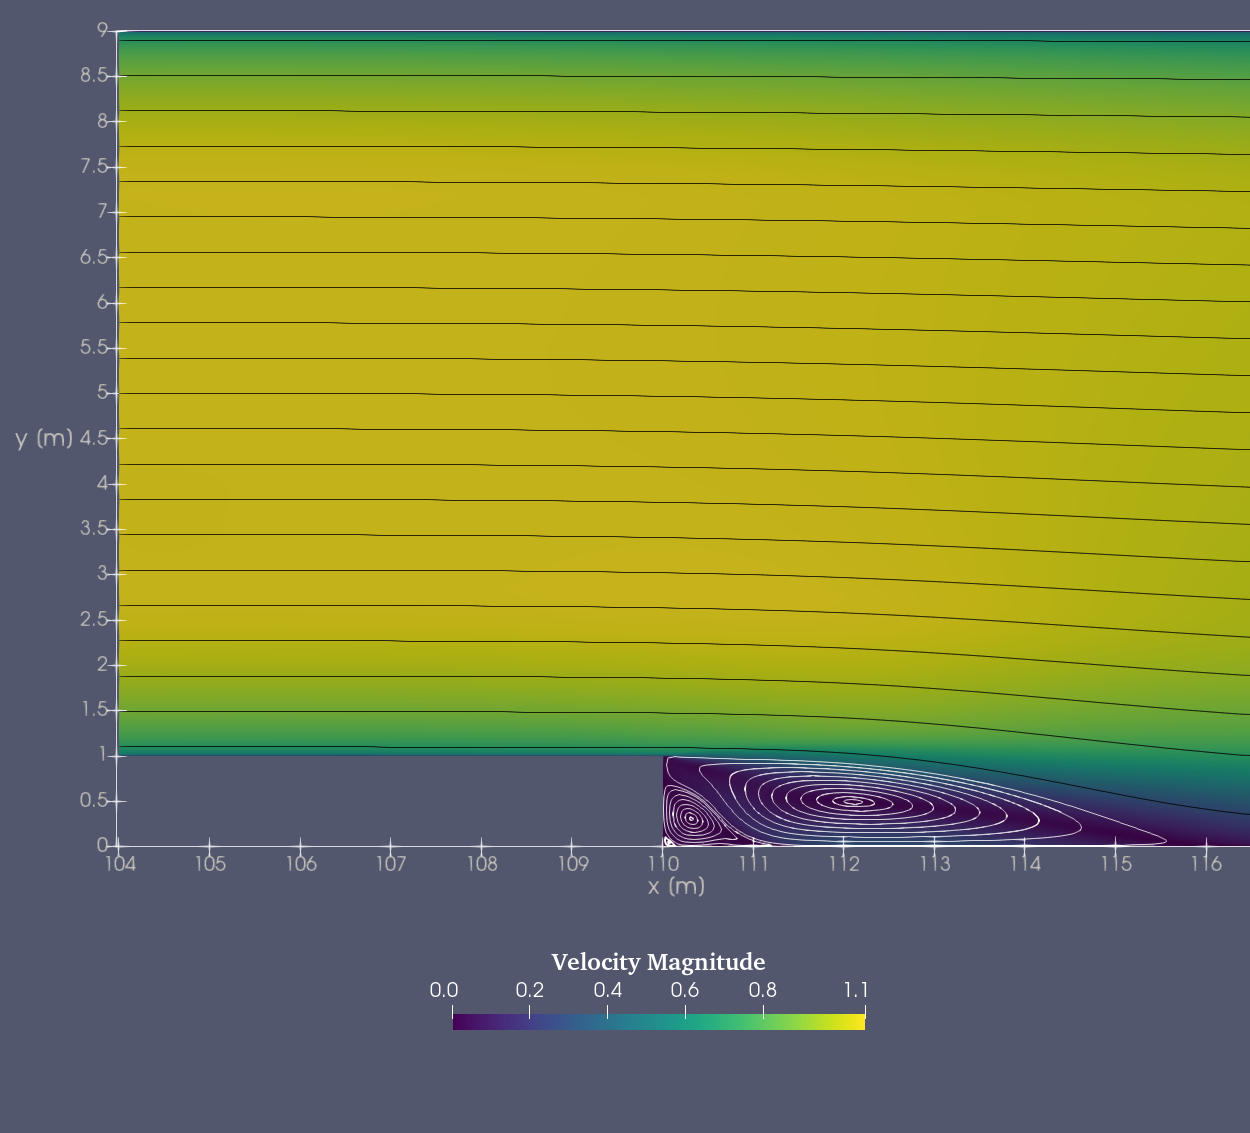
\includegraphics[width=\columnwidth]{bfs}
  \caption{Velocity magnitude distribution and streamlines around the backward-facing step. The
  streamlines illustrate the primary and secondary recirculation zones induced by flow past the
  step.}
  \label{fig:bfs}
\end{figure}

\begin{figure}[htb]
  \centering
  \hfill
  \begin{subfigure}[b]{0.38\columnwidth}
    \centering
    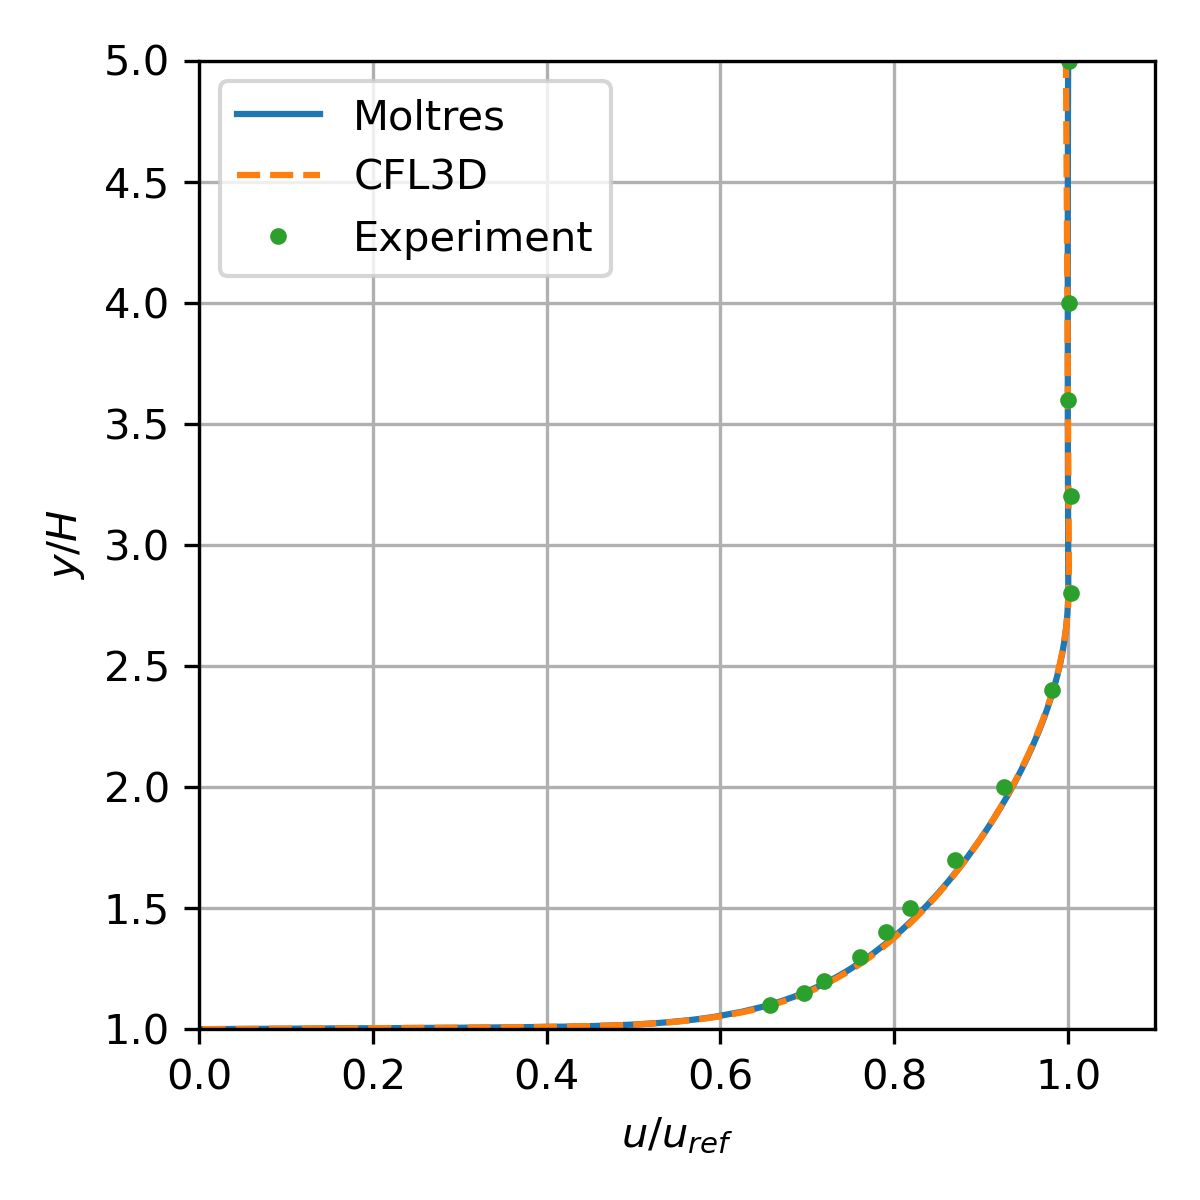
\includegraphics[width=\columnwidth]{bfs_upstream_vel}
    \caption{Normalized velocity distribution at $x/H=-4$ upstream of step.}
    \label{fig:bfs-upstream}
  \end{subfigure}
  \hfill
  \begin{subfigure}[b]{0.38\columnwidth}
    \centering
    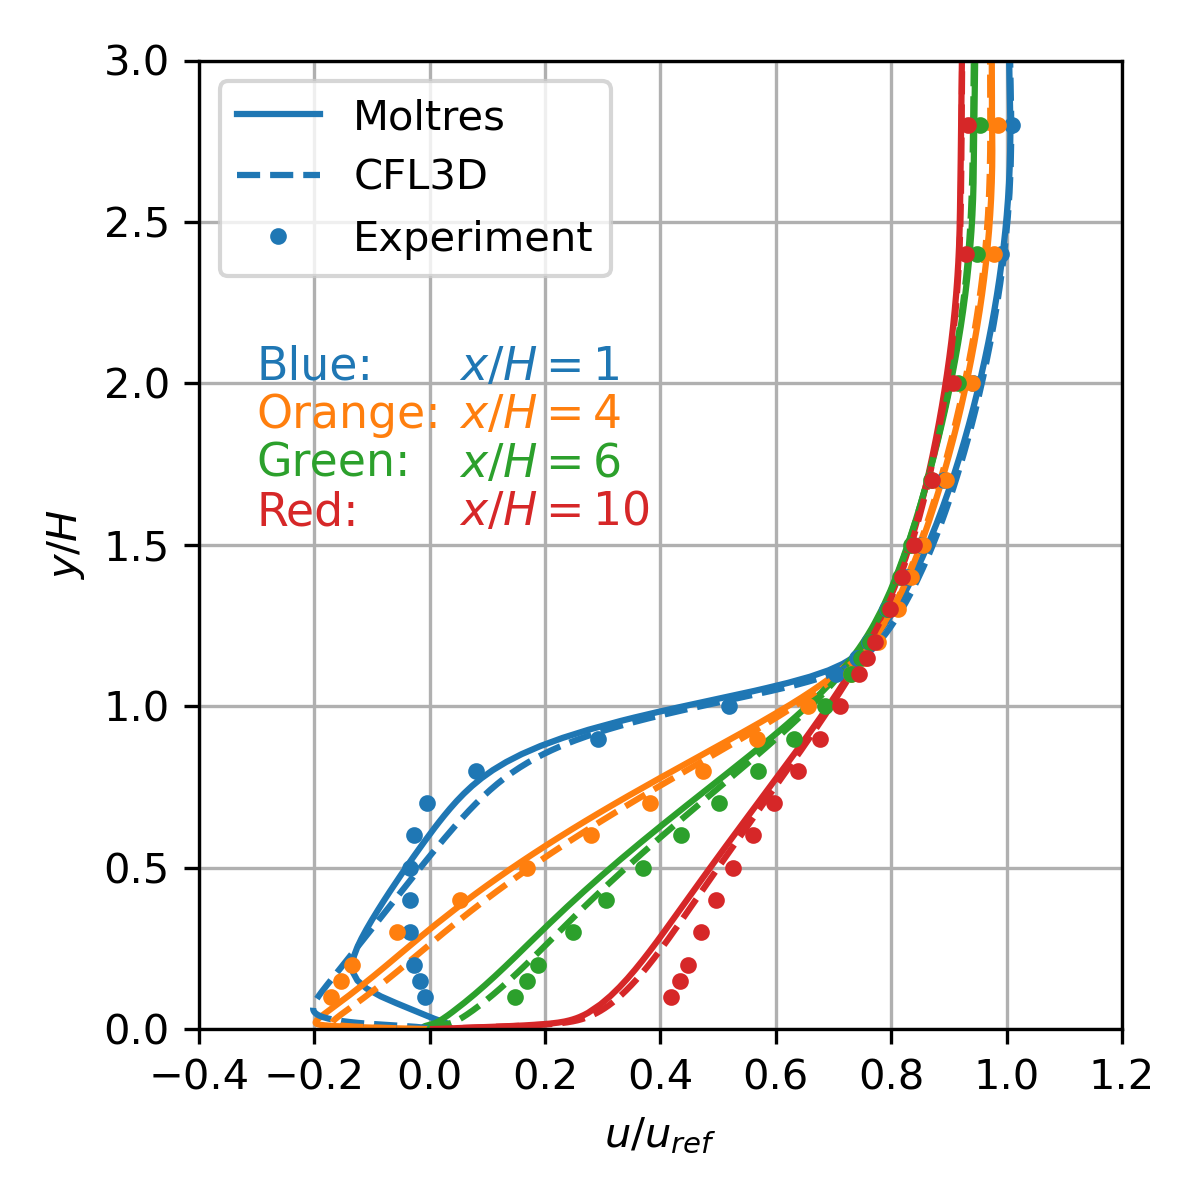
\includegraphics[width=\columnwidth]{bfs_downstream_vel}
    \caption{Normalized velocity distributions downstream of step.}
    \label{fig:bfs-downstream}
  \end{subfigure} \hfill \\
  \centering
  \hfill
  \begin{subfigure}[b]{0.38\columnwidth}
    \centering
    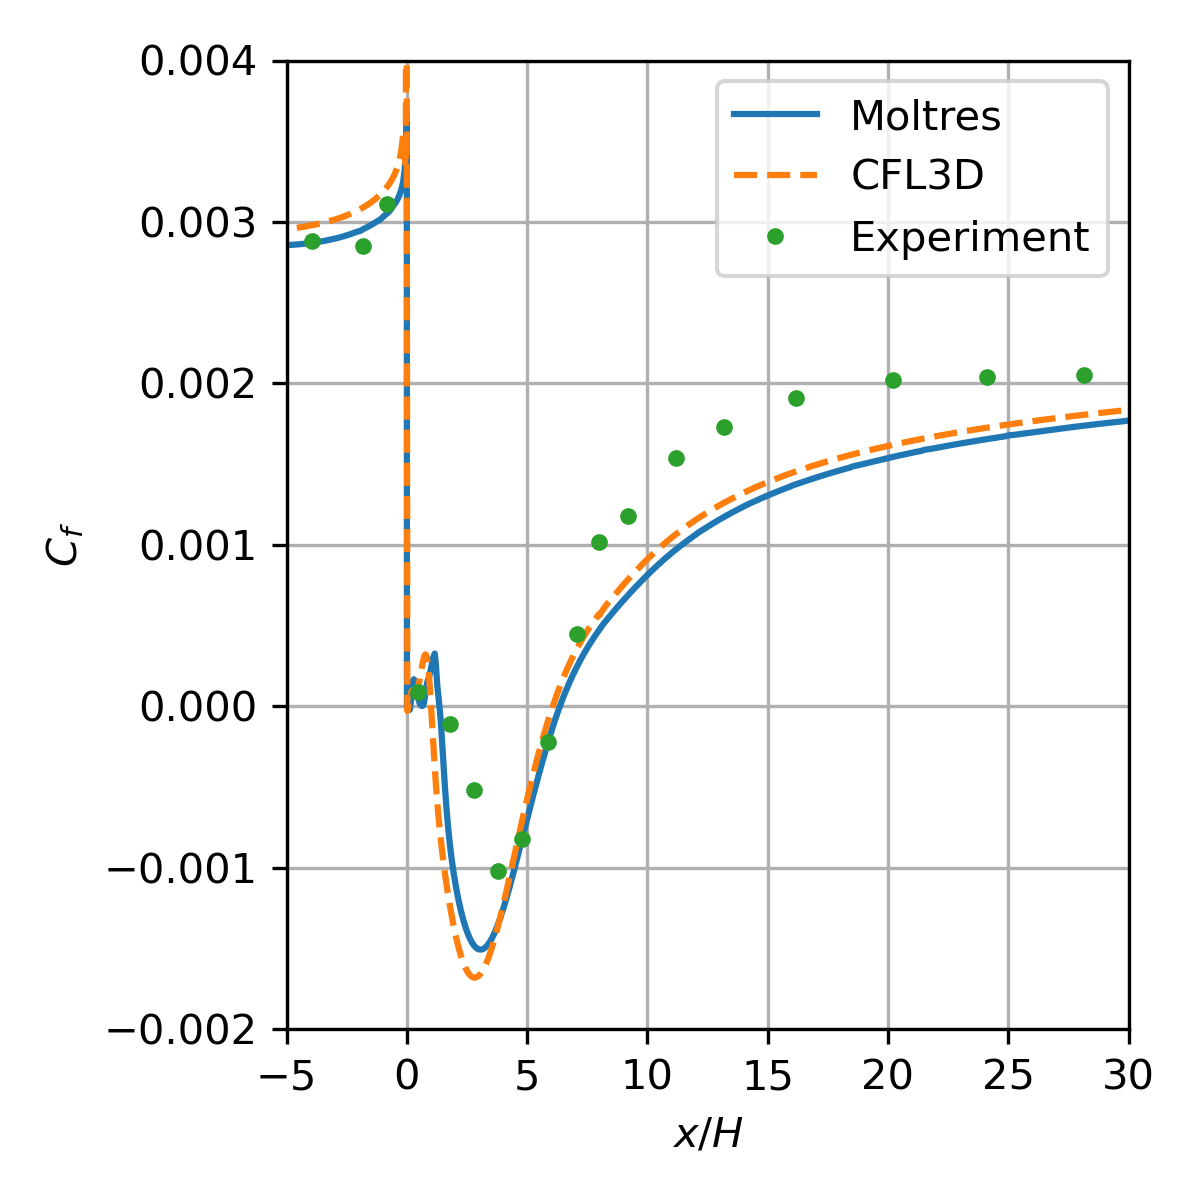
\includegraphics[width=\columnwidth]{bfs_cf}
    \caption{Skin friction coefficient along the bottom wall.}
    \label{fig:bfs-cf}
  \end{subfigure}
  \hfill
  \begin{subfigure}[b]{0.38\columnwidth}
    \centering
    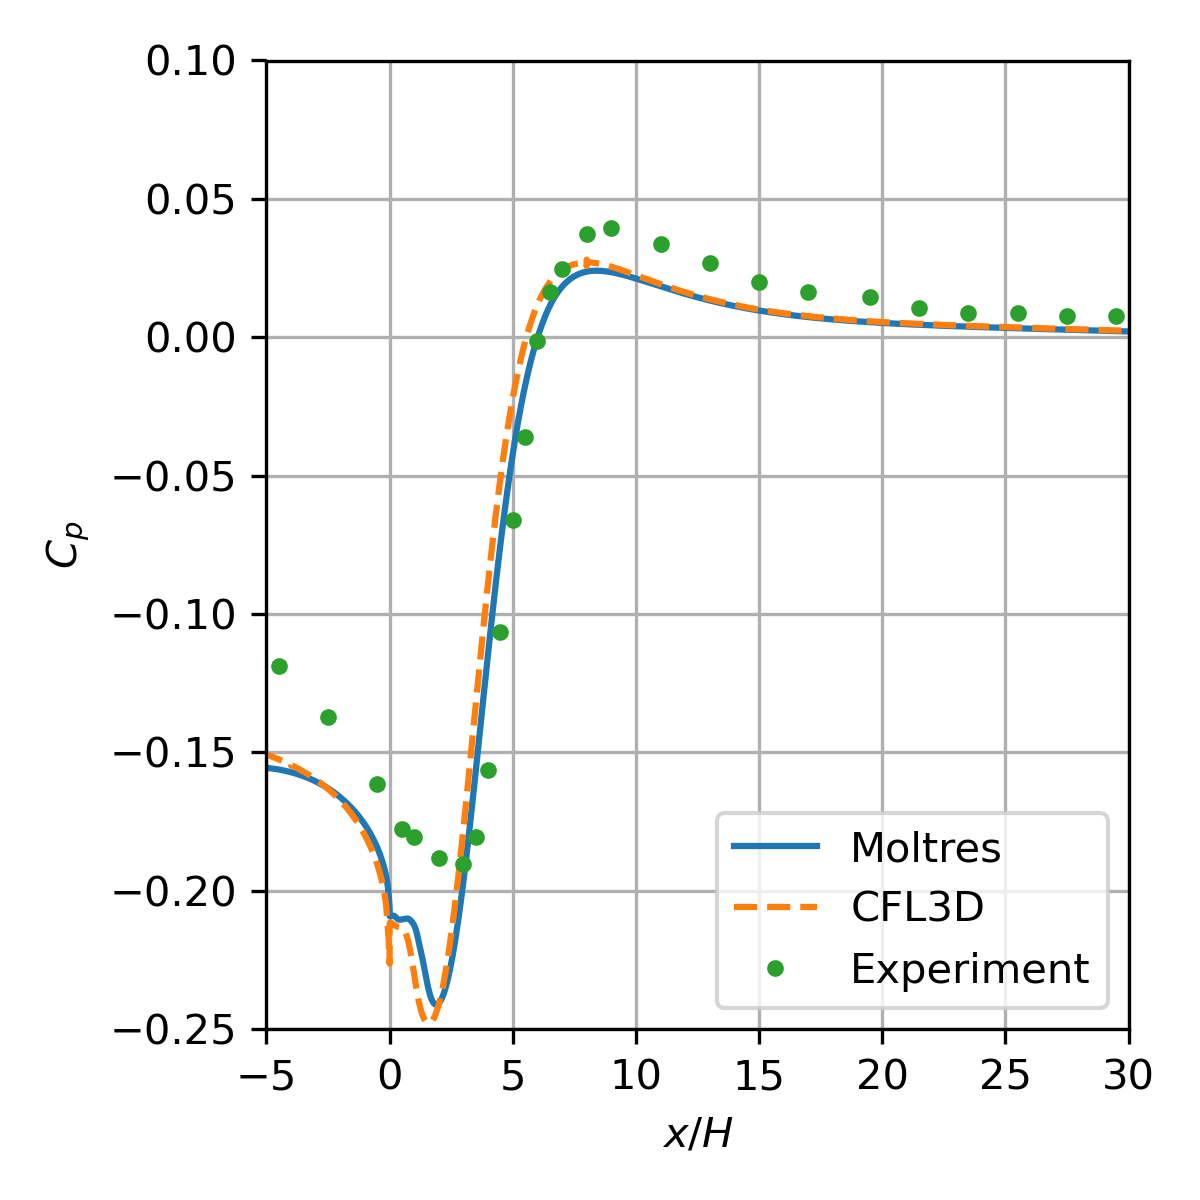
\includegraphics[width=\columnwidth]{bfs_cp}
    \caption{Skin pressure coefficient along the bottom wall.}
    \label{fig:bfs-cp}
  \end{subfigure} \hfill \\
  \centering
  \begin{subfigure}[b]{0.38\columnwidth}
    \centering
    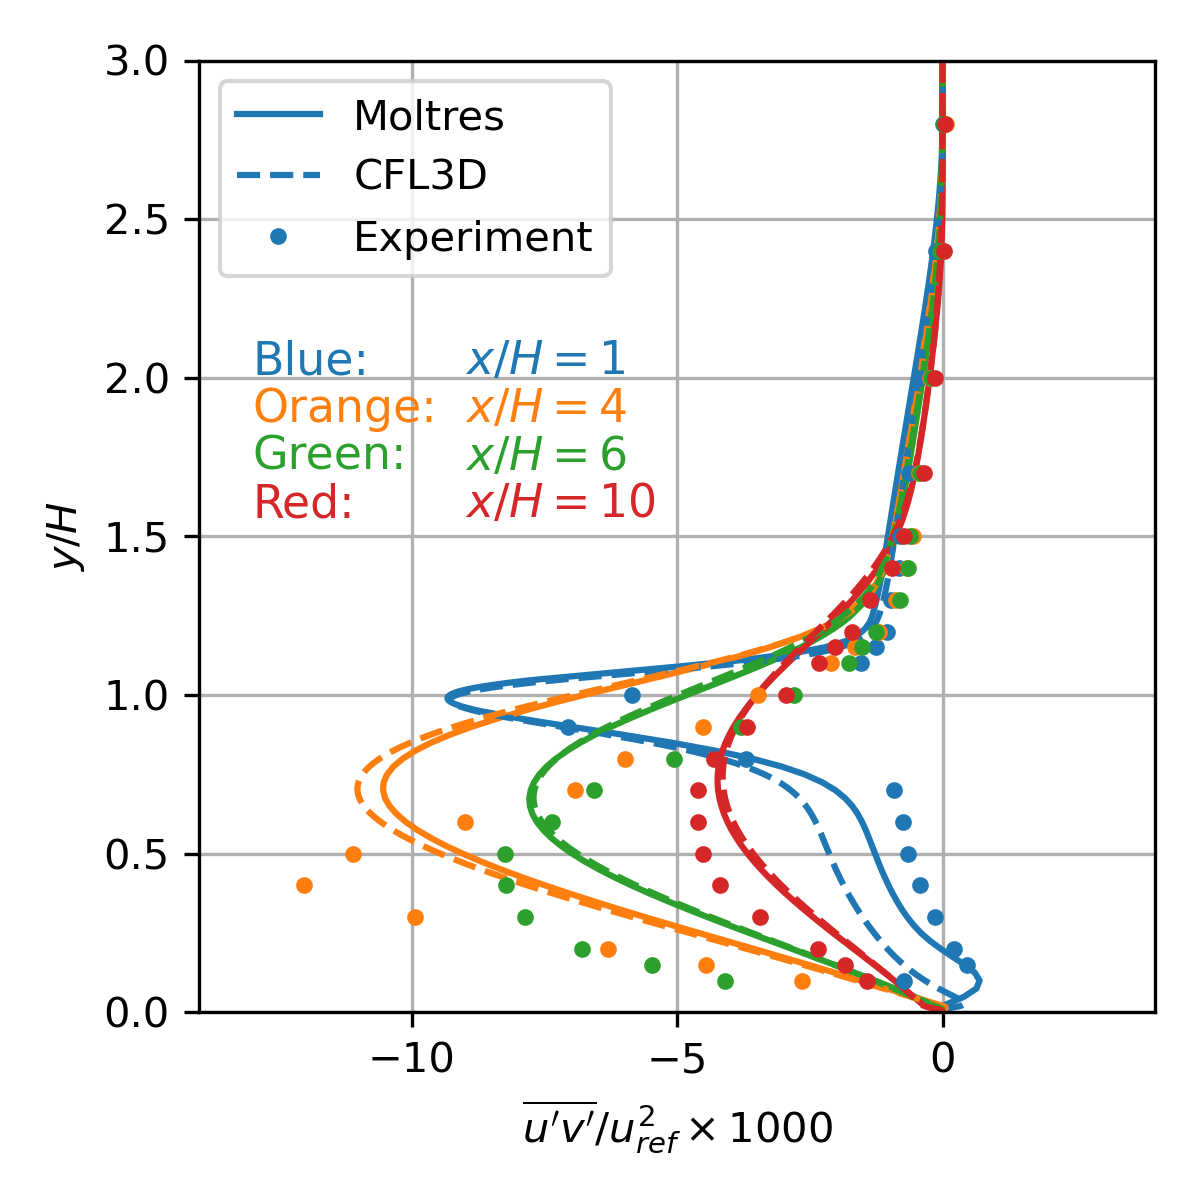
\includegraphics[width=\columnwidth]{bfs_stress}
    \caption{Normalized turbulent shear stress distributions downstream
    of step.}
    \label{fig:bfs-stress}
  \end{subfigure}
  \caption{Comparison of backward facing step flow results against reference
  experimental data and computational data from CFL3D. $x/H$ values are normalized horizontal
  distances relative to the step.}
  \label{fig:bfs-plots}
\end{figure}

\subsection{Summary}

\glspl{MSR} feature turbulent flow along various sections of the primary molten salt loop which in
turn induce turbulent temperature and \glspl{DNP} transport. This section presented the
implementation, verification, and validation of the \gls{SA} turbulence model
\cite{spalart_one-equation_1994} in Moltres for turbulence
modeling capabilities. The one-equation \gls{RANS}-based \gls{SA} model is computationally
efficient relative to more complex \gls{RANS}-based and high-fidelity models while providing better
accuracy than algebraic models when modeling flows with flow separation and significant streamline
curvatures \cite{wilcox_turbulence_2006}.

Verification and validation results for turbulent channel, pipe, and \gls{BFS} flow tests showed
that the Moltres \gls{SA} model is largely consistent with reference simulation or experimental
data in the literature. The Moltres \gls{SA} model includes a rotation correction scheme
\cite{aupoix_extensions_2003, dacles-mariani_numericalexperimental_1995} and notably outperforms
the reference \gls{SA} model in the turbulent \gls{BFS} flow test with more accurate velocity
distributions and flow reattachment length estimate.
